\section{eo\-Pareto\-Fitness\-Traits Class Reference}
\label{classeo_pareto_fitness_traits}\index{eoParetoFitnessTraits@{eoParetoFitnessTraits}}
eo\-Fitness\-Traits: a traits class to specify the number of objectives and which one are maximizing or not See test/t-eo\-Pareto\-Fitness for its use.  


{\tt \#include $<$eo\-Pareto\-Fitness.h$>$}

Inheritance diagram for eo\-Pareto\-Fitness\-Traits::\begin{figure}[H]
\begin{center}
\leavevmode
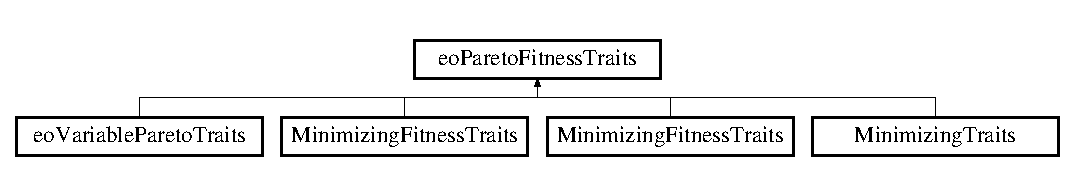
\includegraphics[height=1.86667cm]{classeo_pareto_fitness_traits}
\end{center}
\end{figure}
\subsection*{Static Public Member Functions}
\begin{CompactItemize}
\item 
unsigned {\bf n\-Objectives} ()\label{classeo_pareto_fitness_traits_e0}

\item 
double {\bf tol} ()\label{classeo_pareto_fitness_traits_e1}

\item 
bool {\bf maximizing} (int which)\label{classeo_pareto_fitness_traits_e2}

\end{CompactItemize}


\subsection{Detailed Description}
eo\-Fitness\-Traits: a traits class to specify the number of objectives and which one are maximizing or not See test/t-eo\-Pareto\-Fitness for its use. 

If you define your own, make sure you make the functions static! 



Definition at line 42 of file eo\-Pareto\-Fitness.h.

The documentation for this class was generated from the following file:\begin{CompactItemize}
\item 
eo\-Pareto\-Fitness.h\end{CompactItemize}
